\documentclass[1p]{elsarticle_modified}
%\bibliographystyle{elsarticle-num}

%\usepackage[colorlinks]{hyperref}
%\usepackage{abbrmath_seonhwa} %\Abb, \Ascr, \Acal ,\Abf, \Afrak
\usepackage{amsfonts}
\usepackage{amssymb}
\usepackage{amsmath}
\usepackage{amsthm}
\usepackage{scalefnt}
\usepackage{amsbsy}
\usepackage{kotex}
\usepackage{caption}
\usepackage{subfig}
\usepackage{color}
\usepackage{graphicx}
\usepackage{xcolor} %% white, black, red, green, blue, cyan, magenta, yellow
\usepackage{float}
\usepackage{setspace}
\usepackage{hyperref}

\usepackage{tikz}
\usetikzlibrary{arrows}

\usepackage{multirow}
\usepackage{array} % fixed length table
\usepackage{hhline}

%%%%%%%%%%%%%%%%%%%%%
\makeatletter
\renewcommand*\env@matrix[1][\arraystretch]{%
	\edef\arraystretch{#1}%
	\hskip -\arraycolsep
	\let\@ifnextchar\new@ifnextchar
	\array{*\c@MaxMatrixCols c}}
\makeatother %https://tex.stackexchange.com/questions/14071/how-can-i-increase-the-line-spacing-in-a-matrix
%%%%%%%%%%%%%%%

\usepackage[normalem]{ulem}

\newcommand{\msout}[1]{\ifmmode\text{\sout{\ensuremath{#1}}}\else\sout{#1}\fi}
%SOURCE: \msout is \stkout macro in https://tex.stackexchange.com/questions/20609/strikeout-in-math-mode

\newcommand{\cancel}[1]{
	\ifmmode
	{\color{red}\msout{#1}}
	\else
	{\color{red}\sout{#1}}
	\fi
}

\newcommand{\add}[1]{
	{\color{blue}\uwave{#1}}
}

\newcommand{\replace}[2]{
	\ifmmode
	{\color{red}\msout{#1}}{\color{blue}\uwave{#2}}
	\else
	{\color{red}\sout{#1}}{\color{blue}\uwave{#2}}
	\fi
}

\newcommand{\Sol}{\mathcal{S}} %segment
\newcommand{\D}{D} %diagram
\newcommand{\A}{\mathcal{A}} %arc


%%%%%%%%%%%%%%%%%%%%%%%%%%%%%5 test

\def\sl{\operatorname{\textup{SL}}(2,\Cbb)}
\def\psl{\operatorname{\textup{PSL}}(2,\Cbb)}
\def\quan{\mkern 1mu \triangleright \mkern 1mu}

\theoremstyle{definition}
\newtheorem{thm}{Theorem}[section]
\newtheorem{prop}[thm]{Proposition}
\newtheorem{lem}[thm]{Lemma}
\newtheorem{ques}[thm]{Question}
\newtheorem{cor}[thm]{Corollary}
\newtheorem{defn}[thm]{Definition}
\newtheorem{exam}[thm]{Example}
\newtheorem{rmk}[thm]{Remark}
\newtheorem{alg}[thm]{Algorithm}

\newcommand{\I}{\sqrt{-1}}
\begin{document}

%\begin{frontmatter}
%
%\title{Boundary parabolic representations of knots up to 8 crossings}
%
%%% Group authors per affiliation:
%\author{Yunhi Cho} 
%\address{Department of Mathematics, University of Seoul, Seoul, Korea}
%\ead{yhcho@uos.ac.kr}
%
%
%\author{Seonhwa Kim} %\fnref{s_kim}}
%\address{Center for Geometry and Physics, Institute for Basic Science, Pohang, 37673, Korea}
%\ead{ryeona17@ibs.re.kr}
%
%\author{Hyuk Kim}
%\address{Department of Mathematical Sciences, Seoul National University, Seoul 08826, Korea}
%\ead{hyukkim@snu.ac.kr}
%
%\author{Seokbeom Yoon}
%\address{Department of Mathematical Sciences, Seoul National University, Seoul, 08826,  Korea}
%\ead{sbyoon15@snu.ac.kr}
%
%\begin{abstract}
%We find all boundary parabolic representation of knots up to 8 crossings.
%
%\end{abstract}
%\begin{keyword}
%    \MSC[2010] 57M25 
%\end{keyword}
%
%\end{frontmatter}

%\linenumbers
%\tableofcontents
%
\newcommand\colored[1]{\textcolor{white}{\rule[-0.35ex]{0.8em}{1.4ex}}\kern-0.8em\color{red} #1}%
%\newcommand\colored[1]{\textcolor{white}{ #1}\kern-2.17ex	\textcolor{white}{ #1}\kern-1.81ex	\textcolor{white}{ #1}\kern-2.15ex\color{red}#1	}

{\Large $\underline{12a_{0985}~(K12a_{0985})}$}

\setlength{\tabcolsep}{10pt}
\renewcommand{\arraystretch}{1.6}
\vspace{1cm}\begin{tabular}{m{100pt}>{\centering\arraybackslash}m{274pt}}
\multirow{5}{120pt}{
	\centering
	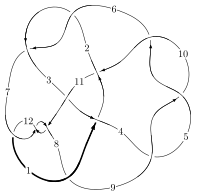
\includegraphics[width=112pt]{../../../GIT/diagram.site/Diagrams/png/1786_12a_0985.png}\\
\ \ \ A knot diagram\footnotemark}&
\allowdisplaybreaks
\textbf{Linearized knot diagam} \\
\cline{2-2}
 &
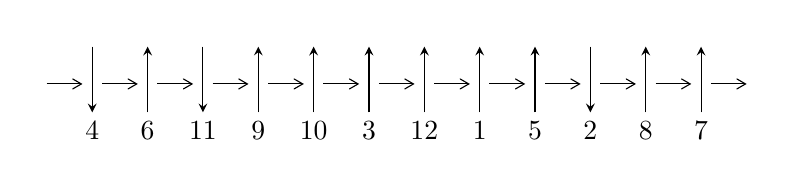
\begin{tikzpicture}[x=20pt, y=17pt]
	% nodes
	\node (C0) at (0, 0) {};
	\node (C1) at (1, 0) {};
	\node (C1U) at (1, +1) {};
	\node (C1D) at (1, -1) {4};

	\node (C2) at (2, 0) {};
	\node (C2U) at (2, +1) {};
	\node (C2D) at (2, -1) {6};

	\node (C3) at (3, 0) {};
	\node (C3U) at (3, +1) {};
	\node (C3D) at (3, -1) {11};

	\node (C4) at (4, 0) {};
	\node (C4U) at (4, +1) {};
	\node (C4D) at (4, -1) {9};

	\node (C5) at (5, 0) {};
	\node (C5U) at (5, +1) {};
	\node (C5D) at (5, -1) {10};

	\node (C6) at (6, 0) {};
	\node (C6U) at (6, +1) {};
	\node (C6D) at (6, -1) {3};

	\node (C7) at (7, 0) {};
	\node (C7U) at (7, +1) {};
	\node (C7D) at (7, -1) {12};

	\node (C8) at (8, 0) {};
	\node (C8U) at (8, +1) {};
	\node (C8D) at (8, -1) {1};

	\node (C9) at (9, 0) {};
	\node (C9U) at (9, +1) {};
	\node (C9D) at (9, -1) {5};

	\node (C10) at (10, 0) {};
	\node (C10U) at (10, +1) {};
	\node (C10D) at (10, -1) {2};

	\node (C11) at (11, 0) {};
	\node (C11U) at (11, +1) {};
	\node (C11D) at (11, -1) {8};

	\node (C12) at (12, 0) {};
	\node (C12U) at (12, +1) {};
	\node (C12D) at (12, -1) {7};
	\node (C13) at (13, 0) {};

	% arrows
	\draw[->,>={angle 60}]
	(C0) edge (C1) (C1) edge (C2) (C2) edge (C3) (C3) edge (C4) (C4) edge (C5) (C5) edge (C6) (C6) edge (C7) (C7) edge (C8) (C8) edge (C9) (C9) edge (C10) (C10) edge (C11) (C11) edge (C12) (C12) edge (C13) ;	\draw[->,>=stealth]
	(C1U) edge (C1D) (C2D) edge (C2U) (C3U) edge (C3D) (C4D) edge (C4U) (C5D) edge (C5U) (C6D) edge (C6U) (C7D) edge (C7U) (C8D) edge (C8U) (C9D) edge (C9U) (C10U) edge (C10D) (C11D) edge (C11U) (C12D) edge (C12U) ;
	\end{tikzpicture} \\
\hhline{~~} \\& 
\textbf{Solving Sequence} \\ \cline{2-2} 
 &
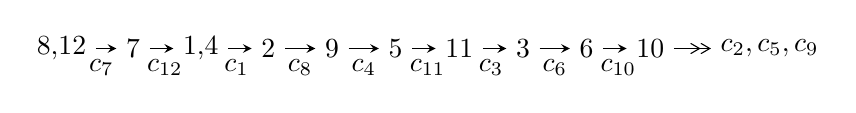
\begin{tikzpicture}[x=23pt, y=7pt]
	% node
	\node (A0) at (-1/8, 0) {8,12};
	\node (A1) at (1, 0) {7};
	\node (A2) at (33/16, 0) {1,4};
	\node (A3) at (25/8, 0) {2};
	\node (A4) at (33/8, 0) {9};
	\node (A5) at (41/8, 0) {5};
	\node (A6) at (49/8, 0) {11};
	\node (A7) at (57/8, 0) {3};
	\node (A8) at (65/8, 0) {6};
	\node (A9) at (73/8, 0) {10};
	\node (C1) at (1/2, -1) {$c_{7}$};
	\node (C2) at (3/2, -1) {$c_{12}$};
	\node (C3) at (21/8, -1) {$c_{1}$};
	\node (C4) at (29/8, -1) {$c_{8}$};
	\node (C5) at (37/8, -1) {$c_{4}$};
	\node (C6) at (45/8, -1) {$c_{11}$};
	\node (C7) at (53/8, -1) {$c_{3}$};
	\node (C8) at (61/8, -1) {$c_{6}$};
	\node (C9) at (69/8, -1) {$c_{10}$};
	\node (A10) at (11, 0) {$c_{2},c_{5},c_{9}$};

	% edge
	\draw[->,>=stealth]	
	(A0) edge (A1) (A1) edge (A2) (A2) edge (A3) (A3) edge (A4) (A4) edge (A5) (A5) edge (A6) (A6) edge (A7) (A7) edge (A8) (A8) edge (A9) ;
	\draw[->>,>={angle 60}]	
	(A9) edge (A10);
\end{tikzpicture} \\ 

\end{tabular} \\

\footnotetext{
The image of knot diagram is generated by the software ``\textbf{Draw programme}" developed by Andrew Bartholomew(\url{http://www.layer8.co.uk/maths/draw/index.htm\#Running-draw}), where we modified some parts for our purpose(\url{https://github.com/CATsTAILs/LinksPainter}).
}\phantom \\ \newline 
\centering \textbf{Ideals for irreducible components\footnotemark of $X_{\text{par}}$} 
 
\begin{align*}
I^u_{1}&=\langle 
3.10359\times10^{88} u^{95}+3.33640\times10^{87} u^{94}+\cdots+3.88345\times10^{88} b-3.40630\times10^{88},\\
\phantom{I^u_{1}}&\phantom{= \langle  }-5.44087\times10^{88} u^{95}-1.88768\times10^{87} u^{94}+\cdots+3.88345\times10^{88} a+4.18452\times10^{89},\\
\phantom{I^u_{1}}&\phantom{= \langle  }u^{96}+41 u^{94}+\cdots+16 u+1\rangle \\
I^u_{2}&=\langle 
-2 u^{17}+2 u^{16}+\cdots+b-1,\;3 u^{17}-4 u^{16}+\cdots+a-4,\;u^{18}- u^{17}+\cdots-5 u-1\rangle \\
\\
\end{align*}
\raggedright * 2 irreducible components of $\dim_{\mathbb{C}}=0$, with total 114 representations.\\
\footnotetext{All coefficients of polynomials are rational numbers. But the coefficients are sometimes approximated in decimal forms when there is not enough margin.}
\newpage
\renewcommand{\arraystretch}{1}
\centering \section*{I. $I^u_{1}= \langle 3.10\times10^{88} u^{95}+3.34\times10^{87} u^{94}+\cdots+3.88\times10^{88} b-3.41\times10^{88},\;-5.44\times10^{88} u^{95}-1.89\times10^{87} u^{94}+\cdots+3.88\times10^{88} a+4.18\times10^{89},\;u^{96}+41 u^{94}+\cdots+16 u+1 \rangle$}
\flushleft \textbf{(i) Arc colorings}\\
\begin{tabular}{m{7pt} m{180pt} m{7pt} m{180pt} }
\flushright $a_{8}=$&$\begin{pmatrix}1\\0\end{pmatrix}$ \\
\flushright $a_{12}=$&$\begin{pmatrix}0\\u\end{pmatrix}$ \\
\flushright $a_{7}=$&$\begin{pmatrix}1\\u^2\end{pmatrix}$ \\
\flushright $a_{1}=$&$\begin{pmatrix}u\\u^3+u\end{pmatrix}$ \\
\flushright $a_{4}=$&$\begin{pmatrix}1.40104 u^{95}+0.0486083 u^{94}+\cdots+15.5984 u-10.7753\\-0.799184 u^{95}-0.0859132 u^{94}+\cdots-9.66228 u+0.877133\end{pmatrix}$ \\
\flushright $a_{2}=$&$\begin{pmatrix}-2.45412 u^{95}-0.730520 u^{94}+\cdots-292.918 u-9.93176\\0.823168 u^{95}+1.17208 u^{94}+\cdots+49.4581 u+2.23074\end{pmatrix}$ \\
\flushright $a_{9}=$&$\begin{pmatrix}- u^4- u^2+1\\- u^6-2 u^4- u^2\end{pmatrix}$ \\
\flushright $a_{5}=$&$\begin{pmatrix}0.876886 u^{95}+0.163384 u^{94}+\cdots+4.35080 u-9.99737\\-0.645493 u^{95}-0.124145 u^{94}+\cdots-9.62974 u+0.878777\end{pmatrix}$ \\
\flushright $a_{11}=$&$\begin{pmatrix}- u\\u\end{pmatrix}$ \\
\flushright $a_{3}=$&$\begin{pmatrix}0.923446 u^{95}+0.0258408 u^{94}+\cdots+15.5935 u-10.7380\\-0.321589 u^{95}-0.0631457 u^{94}+\cdots-9.65730 u+0.839828\end{pmatrix}$ \\
\flushright $a_{6}=$&$\begin{pmatrix}2.16220 u^{95}+0.906974 u^{94}+\cdots+142.246 u-6.51295\\-0.638445 u^{95}-1.57608 u^{94}+\cdots-40.4967 u-0.642127\end{pmatrix}$ \\
\flushright $a_{10}=$&$\begin{pmatrix}-0.695459 u^{95}-0.921443 u^{94}+\cdots-55.8505 u+13.2455\\0.286079 u^{95}+0.128400 u^{94}+\cdots+21.7409 u-0.837753\end{pmatrix}$\\&\end{tabular}
\flushleft \textbf{(ii) Obstruction class $= -1$}\\~\\
\flushleft \textbf{(iii) Cusp Shapes $= -0.146890 u^{95}-0.453328 u^{94}+\cdots-34.2315 u+11.0354$}\\~\\
\newpage\renewcommand{\arraystretch}{1}
\flushleft \textbf{(iv) u-Polynomials at the component}\newline \\
\begin{tabular}{m{50pt}|m{274pt}}
Crossings & \hspace{64pt}u-Polynomials at each crossing \\
\hline $$\begin{aligned}c_{1}\end{aligned}$$&$\begin{aligned}
&u^{96}-16 u^{95}+\cdots+1153236 u-36731
\end{aligned}$\\
\hline $$\begin{aligned}c_{2},c_{6}\end{aligned}$$&$\begin{aligned}
&u^{96}+2 u^{95}+\cdots-1833 u+109
\end{aligned}$\\
\hline $$\begin{aligned}c_{3}\end{aligned}$$&$\begin{aligned}
&u^{96}-2 u^{95}+\cdots-64086 u-9679
\end{aligned}$\\
\hline $$\begin{aligned}c_{4},c_{5},c_{9}\end{aligned}$$&$\begin{aligned}
&u^{96}+2 u^{95}+\cdots+210 u-31
\end{aligned}$\\
\hline $$\begin{aligned}c_{7},c_{11},c_{12}\end{aligned}$$&$\begin{aligned}
&u^{96}+41 u^{94}+\cdots-16 u+1
\end{aligned}$\\
\hline $$\begin{aligned}c_{8}\end{aligned}$$&$\begin{aligned}
&u^{96}-27 u^{94}+\cdots-2362 u+185
\end{aligned}$\\
\hline $$\begin{aligned}c_{10}\end{aligned}$$&$\begin{aligned}
&u^{96}+6 u^{95}+\cdots+575784 u-818513
\end{aligned}$\\
\hline
\end{tabular}\\~\\
\newpage\renewcommand{\arraystretch}{1}
\flushleft \textbf{(v) Riley Polynomials at the component}\newline \\
\begin{tabular}{m{50pt}|m{274pt}}
Crossings & \hspace{64pt}Riley Polynomials at each crossing \\
\hline $$\begin{aligned}c_{1}\end{aligned}$$&$\begin{aligned}
&y^{96}+32 y^{95}+\cdots-717572790842 y+1349166361
\end{aligned}$\\
\hline $$\begin{aligned}c_{2},c_{6}\end{aligned}$$&$\begin{aligned}
&y^{96}-84 y^{95}+\cdots-46507 y+11881
\end{aligned}$\\
\hline $$\begin{aligned}c_{3}\end{aligned}$$&$\begin{aligned}
&y^{96}+24 y^{95}+\cdots+1167091062 y+93683041
\end{aligned}$\\
\hline $$\begin{aligned}c_{4},c_{5},c_{9}\end{aligned}$$&$\begin{aligned}
&y^{96}-104 y^{95}+\cdots-67226 y+961
\end{aligned}$\\
\hline $$\begin{aligned}c_{7},c_{11},c_{12}\end{aligned}$$&$\begin{aligned}
&y^{96}+82 y^{95}+\cdots+134 y+1
\end{aligned}$\\
\hline $$\begin{aligned}c_{8}\end{aligned}$$&$\begin{aligned}
&y^{96}-54 y^{95}+\cdots+4960036 y+34225
\end{aligned}$\\
\hline $$\begin{aligned}c_{10}\end{aligned}$$&$\begin{aligned}
&y^{96}+44 y^{95}+\cdots+6891789440382 y+669963531169
\end{aligned}$\\
\hline
\end{tabular}\\~\\
\newpage\flushleft \textbf{(vi) Complex Volumes and Cusp Shapes}
$$\begin{array}{c|c|c}  
\text{Solutions to }I^u_{1}& \I (\text{vol} + \sqrt{-1}CS) & \text{Cusp shape}\\
 \hline 
\begin{aligned}
u &= \phantom{-}0.297798 + 0.927894 I \\
a &= \phantom{-}1.42481 + 0.33774 I \\
b &= -1.048500 + 0.528138 I\end{aligned}
 & \phantom{-}5.33002 + 2.05817 I & \phantom{-0.000000 } 0 \\ \hline\begin{aligned}
u &= \phantom{-}0.297798 - 0.927894 I \\
a &= \phantom{-}1.42481 - 0.33774 I \\
b &= -1.048500 - 0.528138 I\end{aligned}
 & \phantom{-}5.33002 - 2.05817 I & \phantom{-0.000000 } 0 \\ \hline\begin{aligned}
u &= -0.242954 + 0.935876 I \\
a &= \phantom{-}1.67582 + 1.00350 I \\
b &= -0.922321 - 0.576315 I\end{aligned}
 & \phantom{-}5.33582 + 2.30326 I & \phantom{-0.000000 } 0 \\ \hline\begin{aligned}
u &= -0.242954 - 0.935876 I \\
a &= \phantom{-}1.67582 - 1.00350 I \\
b &= -0.922321 + 0.576315 I\end{aligned}
 & \phantom{-}5.33582 - 2.30326 I & \phantom{-0.000000 } 0 \\ \hline\begin{aligned}
u &= -0.468863 + 0.815205 I \\
a &= \phantom{-}0.884133 - 0.393898 I \\
b &= -0.149099 - 0.185872 I\end{aligned}
 & \phantom{-}2.77482 - 3.30617 I & \phantom{-0.000000 } 0 \\ \hline\begin{aligned}
u &= -0.468863 - 0.815205 I \\
a &= \phantom{-}0.884133 + 0.393898 I \\
b &= -0.149099 + 0.185872 I\end{aligned}
 & \phantom{-}2.77482 + 3.30617 I & \phantom{-0.000000 } 0 \\ \hline\begin{aligned}
u &= \phantom{-}0.368372 + 0.999484 I \\
a &= \phantom{-}1.32514 - 1.17194 I \\
b &= \phantom{-}0.063016 + 1.038760 I\end{aligned}
 & \phantom{-}3.41807 - 4.04230 I & \phantom{-0.000000 } 0 \\ \hline\begin{aligned}
u &= \phantom{-}0.368372 - 0.999484 I \\
a &= \phantom{-}1.32514 + 1.17194 I \\
b &= \phantom{-}0.063016 - 1.038760 I\end{aligned}
 & \phantom{-}3.41807 + 4.04230 I & \phantom{-0.000000 } 0 \\ \hline\begin{aligned}
u &= \phantom{-}1.028350 + 0.284393 I \\
a &= -0.0242050 + 0.0238082 I \\
b &= \phantom{-}0.202927 - 0.715178 I\end{aligned}
 & \phantom{-}11.15810 + 1.10966 I & \phantom{-0.000000 } 0 \\ \hline\begin{aligned}
u &= \phantom{-}1.028350 - 0.284393 I \\
a &= -0.0242050 - 0.0238082 I \\
b &= \phantom{-}0.202927 + 0.715178 I\end{aligned}
 & \phantom{-}11.15810 - 1.10966 I & \phantom{-0.000000 } 0\\
 \hline 
 \end{array}$$\newpage$$\begin{array}{c|c|c}  
\text{Solutions to }I^u_{1}& \I (\text{vol} + \sqrt{-1}CS) & \text{Cusp shape}\\
 \hline 
\begin{aligned}
u &= -0.876854 + 0.192713 I \\
a &= \phantom{-}0.0135335 - 0.0501523 I \\
b &= \phantom{-}0.75480 + 1.70626 I\end{aligned}
 & \phantom{-}13.6016 - 12.2540 I & \phantom{-}13.3299 + 6.6530 I \\ \hline\begin{aligned}
u &= -0.876854 - 0.192713 I \\
a &= \phantom{-}0.0135335 + 0.0501523 I \\
b &= \phantom{-}0.75480 - 1.70626 I\end{aligned}
 & \phantom{-}13.6016 + 12.2540 I & \phantom{-}13.3299 - 6.6530 I \\ \hline\begin{aligned}
u &= -0.858239 + 0.247052 I \\
a &= -0.135607 - 0.107341 I \\
b &= -0.049923 - 0.793801 I\end{aligned}
 & \phantom{-}4.65285 - 1.38450 I & \phantom{-}21.4925 + 3.3160 I \\ \hline\begin{aligned}
u &= -0.858239 - 0.247052 I \\
a &= -0.135607 + 0.107341 I \\
b &= -0.049923 + 0.793801 I\end{aligned}
 & \phantom{-}4.65285 + 1.38450 I & \phantom{-}21.4925 - 3.3160 I \\ \hline\begin{aligned}
u &= \phantom{-}0.754888 + 0.867470 I \\
a &= -0.579279 - 0.114684 I \\
b &= \phantom{-}0.177260 - 0.377626 I\end{aligned}
 & \phantom{-}9.34632 + 4.89597 I & \phantom{-0.000000 } 0 \\ \hline\begin{aligned}
u &= \phantom{-}0.754888 - 0.867470 I \\
a &= -0.579279 + 0.114684 I \\
b &= \phantom{-}0.177260 + 0.377626 I\end{aligned}
 & \phantom{-}9.34632 - 4.89597 I & \phantom{-0.000000 } 0 \\ \hline\begin{aligned}
u &= -0.037077 + 1.150490 I \\
a &= \phantom{-}2.41494 + 0.68901 I \\
b &= -2.26468 - 0.22862 I\end{aligned}
 & \phantom{-}5.51141 + 2.29478 I & \phantom{-0.000000 } 0 \\ \hline\begin{aligned}
u &= -0.037077 - 1.150490 I \\
a &= \phantom{-}2.41494 - 0.68901 I \\
b &= -2.26468 + 0.22862 I\end{aligned}
 & \phantom{-}5.51141 - 2.29478 I & \phantom{-0.000000 } 0 \\ \hline\begin{aligned}
u &= -0.506526 + 1.045940 I \\
a &= -1.10492 - 1.20836 I \\
b &= -0.137683 + 1.058590 I\end{aligned}
 & \phantom{-}10.99120 + 7.36565 I & \phantom{-0.000000 } 0 \\ \hline\begin{aligned}
u &= -0.506526 - 1.045940 I \\
a &= -1.10492 + 1.20836 I \\
b &= -0.137683 - 1.058590 I\end{aligned}
 & \phantom{-}10.99120 - 7.36565 I & \phantom{-0.000000 } 0\\
 \hline 
 \end{array}$$\newpage$$\begin{array}{c|c|c}  
\text{Solutions to }I^u_{1}& \I (\text{vol} + \sqrt{-1}CS) & \text{Cusp shape}\\
 \hline 
\begin{aligned}
u &= \phantom{-}0.803111 + 0.179218 I \\
a &= -0.066784 + 0.203569 I \\
b &= -0.72208 + 1.76413 I\end{aligned}
 & \phantom{-}5.96033 + 8.31880 I & \phantom{-}11.72121 - 7.68923 I \\ \hline\begin{aligned}
u &= \phantom{-}0.803111 - 0.179218 I \\
a &= -0.066784 - 0.203569 I \\
b &= -0.72208 - 1.76413 I\end{aligned}
 & \phantom{-}5.96033 - 8.31880 I & \phantom{-}11.72121 + 7.68923 I \\ \hline\begin{aligned}
u &= \phantom{-}0.799970 + 0.191989 I \\
a &= \phantom{-}0.402602 - 0.223941 I \\
b &= \phantom{-}0.393651 + 0.967532 I\end{aligned}
 & \phantom{-}7.69465 + 2.08742 I & \phantom{-}12.33446 + 0. I\phantom{ +0.000000I} \\ \hline\begin{aligned}
u &= \phantom{-}0.799970 - 0.191989 I \\
a &= \phantom{-}0.402602 + 0.223941 I \\
b &= \phantom{-}0.393651 - 0.967532 I\end{aligned}
 & \phantom{-}7.69465 - 2.08742 I & \phantom{-}12.33446 + 0. I\phantom{ +0.000000I} \\ \hline\begin{aligned}
u &= -0.765641 + 0.177569 I \\
a &= \phantom{-}0.058867 + 0.521809 I \\
b &= -0.49997 - 1.70099 I\end{aligned}
 & \phantom{-}7.76985 - 6.20036 I & \phantom{-}12.5527 + 7.0916 I \\ \hline\begin{aligned}
u &= -0.765641 - 0.177569 I \\
a &= \phantom{-}0.058867 - 0.521809 I \\
b &= -0.49997 + 1.70099 I\end{aligned}
 & \phantom{-}7.76985 + 6.20036 I & \phantom{-}12.5527 - 7.0916 I \\ \hline\begin{aligned}
u &= \phantom{-}0.174399 + 1.204260 I \\
a &= -1.41191 + 1.18471 I \\
b &= \phantom{-}0.94890 - 1.10675 I\end{aligned}
 & -1.78673 - 0.55616 I & \phantom{-0.000000 } 0 \\ \hline\begin{aligned}
u &= \phantom{-}0.174399 - 1.204260 I \\
a &= -1.41191 - 1.18471 I \\
b &= \phantom{-}0.94890 + 1.10675 I\end{aligned}
 & -1.78673 + 0.55616 I & \phantom{-0.000000 } 0 \\ \hline\begin{aligned}
u &= -0.260942 + 1.195980 I \\
a &= -1.60099 - 1.89265 I \\
b &= -0.13554 + 1.56039 I\end{aligned}
 & \phantom{-}1.76493 - 1.30510 I & \phantom{-0.000000 } 0 \\ \hline\begin{aligned}
u &= -0.260942 - 1.195980 I \\
a &= -1.60099 + 1.89265 I \\
b &= -0.13554 - 1.56039 I\end{aligned}
 & \phantom{-}1.76493 + 1.30510 I & \phantom{-0.000000 } 0\\
 \hline 
 \end{array}$$\newpage$$\begin{array}{c|c|c}  
\text{Solutions to }I^u_{1}& \I (\text{vol} + \sqrt{-1}CS) & \text{Cusp shape}\\
 \hline 
\begin{aligned}
u &= \phantom{-}0.248016 + 1.217990 I \\
a &= -2.02802 + 0.13854 I \\
b &= \phantom{-}1.116670 - 0.085813 I\end{aligned}
 & \phantom{-}1.48638 + 1.59400 I & \phantom{-0.000000 } 0 \\ \hline\begin{aligned}
u &= \phantom{-}0.248016 - 1.217990 I \\
a &= -2.02802 - 0.13854 I \\
b &= \phantom{-}1.116670 + 0.085813 I\end{aligned}
 & \phantom{-}1.48638 - 1.59400 I & \phantom{-0.000000 } 0 \\ \hline\begin{aligned}
u &= \phantom{-}0.751595 + 0.016937 I \\
a &= -1.059530 - 0.071636 I \\
b &= -1.02361 - 1.53401 I\end{aligned}
 & \phantom{-}12.26790 + 3.03497 I & \phantom{-}16.1617 - 2.7279 I \\ \hline\begin{aligned}
u &= \phantom{-}0.751595 - 0.016937 I \\
a &= -1.059530 + 0.071636 I \\
b &= -1.02361 + 1.53401 I\end{aligned}
 & \phantom{-}12.26790 - 3.03497 I & \phantom{-}16.1617 + 2.7279 I \\ \hline\begin{aligned}
u &= -0.021473 + 1.257070 I \\
a &= \phantom{-}2.41435 - 0.48914 I \\
b &= -1.28386 + 0.71695 I\end{aligned}
 & \phantom{-}4.59269 - 2.78319 I & \phantom{-0.000000 } 0 \\ \hline\begin{aligned}
u &= -0.021473 - 1.257070 I \\
a &= \phantom{-}2.41435 + 0.48914 I \\
b &= -1.28386 - 0.71695 I\end{aligned}
 & \phantom{-}4.59269 + 2.78319 I & \phantom{-0.000000 } 0 \\ \hline\begin{aligned}
u &= -0.732032 + 0.098973 I \\
a &= \phantom{-}0.483559 + 0.553909 I \\
b &= \phantom{-}0.89041 + 1.93513 I\end{aligned}
 & \phantom{-}5.04928 - 2.30450 I & \phantom{-}15.6170 + 4.0427 I \\ \hline\begin{aligned}
u &= -0.732032 - 0.098973 I \\
a &= \phantom{-}0.483559 - 0.553909 I \\
b &= \phantom{-}0.89041 - 1.93513 I\end{aligned}
 & \phantom{-}5.04928 + 2.30450 I & \phantom{-}15.6170 - 4.0427 I \\ \hline\begin{aligned}
u &= -0.731589 + 0.019018 I \\
a &= -1.205440 - 0.361661 I \\
b &= \phantom{-}0.61819 + 1.51176 I\end{aligned}
 & \phantom{-}11.74330 + 2.07260 I & \phantom{-}17.0633 - 3.3447 I \\ \hline\begin{aligned}
u &= -0.731589 - 0.019018 I \\
a &= -1.205440 + 0.361661 I \\
b &= \phantom{-}0.61819 - 1.51176 I\end{aligned}
 & \phantom{-}11.74330 - 2.07260 I & \phantom{-}17.0633 + 3.3447 I\\
 \hline 
 \end{array}$$\newpage$$\begin{array}{c|c|c}  
\text{Solutions to }I^u_{1}& \I (\text{vol} + \sqrt{-1}CS) & \text{Cusp shape}\\
 \hline 
\begin{aligned}
u &= \phantom{-}0.703785 + 0.084147 I \\
a &= \phantom{-}0.813100 - 0.049463 I \\
b &= -0.379016 - 1.165570 I\end{aligned}
 & \phantom{-}4.89946 + 1.84798 I & \phantom{-}17.8296 - 4.2620 I \\ \hline\begin{aligned}
u &= \phantom{-}0.703785 - 0.084147 I \\
a &= \phantom{-}0.813100 + 0.049463 I \\
b &= -0.379016 + 1.165570 I\end{aligned}
 & \phantom{-}4.89946 - 1.84798 I & \phantom{-}17.8296 + 4.2620 I \\ \hline\begin{aligned}
u &= \phantom{-}0.695883 + 0.132592 I \\
a &= -0.033172 + 0.207088 I \\
b &= \phantom{-}0.58544 - 1.43059 I\end{aligned}
 & \phantom{-}1.24016 + 3.72681 I & \phantom{-}8.54039 - 7.95601 I \\ \hline\begin{aligned}
u &= \phantom{-}0.695883 - 0.132592 I \\
a &= -0.033172 - 0.207088 I \\
b &= \phantom{-}0.58544 + 1.43059 I\end{aligned}
 & \phantom{-}1.24016 - 3.72681 I & \phantom{-}8.54039 + 7.95601 I \\ \hline\begin{aligned}
u &= -0.295356 + 1.258260 I \\
a &= -0.82981 - 2.24049 I \\
b &= \phantom{-}0.46143 + 2.69377 I\end{aligned}
 & \phantom{-}7.91422 - 5.77924 I & \phantom{-0.000000 } 0 \\ \hline\begin{aligned}
u &= -0.295356 - 1.258260 I \\
a &= -0.82981 + 2.24049 I \\
b &= \phantom{-}0.46143 - 2.69377 I\end{aligned}
 & \phantom{-}7.91422 + 5.77924 I & \phantom{-0.000000 } 0 \\ \hline\begin{aligned}
u &= \phantom{-}0.310058 + 1.254940 I \\
a &= -2.05810 + 0.49235 I \\
b &= \phantom{-}1.67334 - 1.92790 I\end{aligned}
 & \phantom{-}8.44313 + 0.79707 I & \phantom{-0.000000 } 0 \\ \hline\begin{aligned}
u &= \phantom{-}0.310058 - 1.254940 I \\
a &= -2.05810 - 0.49235 I \\
b &= \phantom{-}1.67334 + 1.92790 I\end{aligned}
 & \phantom{-}8.44313 - 0.79707 I & \phantom{-0.000000 } 0 \\ \hline\begin{aligned}
u &= -0.136050 + 1.299620 I \\
a &= \phantom{-}0.328660 - 0.105995 I \\
b &= -0.612886 - 1.001880 I\end{aligned}
 & -4.03722 - 1.90716 I & \phantom{-0.000000 } 0 \\ \hline\begin{aligned}
u &= -0.136050 - 1.299620 I \\
a &= \phantom{-}0.328660 + 0.105995 I \\
b &= -0.612886 + 1.001880 I\end{aligned}
 & -4.03722 + 1.90716 I & \phantom{-0.000000 } 0\\
 \hline 
 \end{array}$$\newpage$$\begin{array}{c|c|c}  
\text{Solutions to }I^u_{1}& \I (\text{vol} + \sqrt{-1}CS) & \text{Cusp shape}\\
 \hline 
\begin{aligned}
u &= -0.252390 + 1.285990 I \\
a &= -2.21302 - 0.29107 I \\
b &= \phantom{-}1.70487 + 1.10185 I\end{aligned}
 & -2.67540 - 3.29908 I & \phantom{-0.000000 } 0 \\ \hline\begin{aligned}
u &= -0.252390 - 1.285990 I \\
a &= -2.21302 + 0.29107 I \\
b &= \phantom{-}1.70487 - 1.10185 I\end{aligned}
 & -2.67540 + 3.29908 I & \phantom{-0.000000 } 0 \\ \hline\begin{aligned}
u &= \phantom{-}0.316404 + 1.278790 I \\
a &= \phantom{-}0.79569 - 1.82844 I \\
b &= \phantom{-}0.599041 + 1.059650 I\end{aligned}
 & \phantom{-}8.23786 + 6.89090 I & \phantom{-0.000000 } 0 \\ \hline\begin{aligned}
u &= \phantom{-}0.316404 - 1.278790 I \\
a &= \phantom{-}0.79569 + 1.82844 I \\
b &= \phantom{-}0.599041 - 1.059650 I\end{aligned}
 & \phantom{-}8.23786 - 6.89090 I & \phantom{-0.000000 } 0 \\ \hline\begin{aligned}
u &= -0.303533 + 1.283320 I \\
a &= \phantom{-}2.23154 + 0.38372 I \\
b &= -1.361510 - 0.277434 I\end{aligned}
 & \phantom{-}7.68745 - 1.66728 I & \phantom{-0.000000 } 0 \\ \hline\begin{aligned}
u &= -0.303533 - 1.283320 I \\
a &= \phantom{-}2.23154 - 0.38372 I \\
b &= -1.361510 + 0.277434 I\end{aligned}
 & \phantom{-}7.68745 + 1.66728 I & \phantom{-0.000000 } 0 \\ \hline\begin{aligned}
u &= -0.248832 + 1.313700 I \\
a &= \phantom{-}1.09035 + 0.97321 I \\
b &= -0.486336 - 1.022820 I\end{aligned}
 & -2.86852 - 3.08123 I & \phantom{-0.000000 } 0 \\ \hline\begin{aligned}
u &= -0.248832 - 1.313700 I \\
a &= \phantom{-}1.09035 - 0.97321 I \\
b &= -0.486336 + 1.022820 I\end{aligned}
 & -2.86852 + 3.08123 I & \phantom{-0.000000 } 0 \\ \hline\begin{aligned}
u &= -0.025099 + 1.349610 I \\
a &= -1.092790 + 0.441049 I \\
b &= \phantom{-}1.385700 + 0.275464 I\end{aligned}
 & -3.10973 - 0.12051 I & \phantom{-0.000000 } 0 \\ \hline\begin{aligned}
u &= -0.025099 - 1.349610 I \\
a &= -1.092790 - 0.441049 I \\
b &= \phantom{-}1.385700 - 0.275464 I\end{aligned}
 & -3.10973 + 0.12051 I & \phantom{-0.000000 } 0\\
 \hline 
 \end{array}$$\newpage$$\begin{array}{c|c|c}  
\text{Solutions to }I^u_{1}& \I (\text{vol} + \sqrt{-1}CS) & \text{Cusp shape}\\
 \hline 
\begin{aligned}
u &= \phantom{-}0.289627 + 1.322520 I \\
a &= \phantom{-}0.77601 - 1.37242 I \\
b &= -0.42944 + 1.89136 I\end{aligned}
 & \phantom{-}0.47824 + 5.45167 I & \phantom{-0.000000 } 0 \\ \hline\begin{aligned}
u &= \phantom{-}0.289627 - 1.322520 I \\
a &= \phantom{-}0.77601 + 1.37242 I \\
b &= -0.42944 - 1.89136 I\end{aligned}
 & \phantom{-}0.47824 - 5.45167 I & \phantom{-0.000000 } 0 \\ \hline\begin{aligned}
u &= -0.309892 + 1.329500 I \\
a &= \phantom{-}2.44045 + 0.85201 I \\
b &= -1.61454 - 2.21245 I\end{aligned}
 & \phantom{-}0.55606 - 6.08308 I & \phantom{-0.000000 } 0 \\ \hline\begin{aligned}
u &= -0.309892 - 1.329500 I \\
a &= \phantom{-}2.44045 - 0.85201 I \\
b &= -1.61454 + 2.21245 I\end{aligned}
 & \phantom{-}0.55606 + 6.08308 I & \phantom{-0.000000 } 0 \\ \hline\begin{aligned}
u &= -0.633892 + 0.010730 I \\
a &= -0.253223 + 0.050010 I \\
b &= -0.579715 + 1.054560 I\end{aligned}
 & \phantom{-}1.320770 + 0.084987 I & \phantom{-}9.06513 + 0.40515 I \\ \hline\begin{aligned}
u &= -0.633892 - 0.010730 I \\
a &= -0.253223 - 0.050010 I \\
b &= -0.579715 - 1.054560 I\end{aligned}
 & \phantom{-}1.320770 - 0.084987 I & \phantom{-}9.06513 - 0.40515 I \\ \hline\begin{aligned}
u &= \phantom{-}0.042448 + 1.371830 I \\
a &= \phantom{-}0.271221 + 0.211770 I \\
b &= -0.006035 - 0.968999 I\end{aligned}
 & -6.65383 - 0.57803 I & \phantom{-0.000000 } 0 \\ \hline\begin{aligned}
u &= \phantom{-}0.042448 - 1.371830 I \\
a &= \phantom{-}0.271221 - 0.211770 I \\
b &= -0.006035 + 0.968999 I\end{aligned}
 & -6.65383 + 0.57803 I & \phantom{-0.000000 } 0 \\ \hline\begin{aligned}
u &= \phantom{-}0.292775 + 1.342320 I \\
a &= \phantom{-}2.23024 - 0.79047 I \\
b &= -1.68849 + 1.44385 I\end{aligned}
 & -3.40813 + 7.33110 I & \phantom{-0.000000 } 0 \\ \hline\begin{aligned}
u &= \phantom{-}0.292775 - 1.342320 I \\
a &= \phantom{-}2.23024 + 0.79047 I \\
b &= -1.68849 - 1.44385 I\end{aligned}
 & -3.40813 - 7.33110 I & \phantom{-0.000000 } 0\\
 \hline 
 \end{array}$$\newpage$$\begin{array}{c|c|c}  
\text{Solutions to }I^u_{1}& \I (\text{vol} + \sqrt{-1}CS) & \text{Cusp shape}\\
 \hline 
\begin{aligned}
u &= -0.323456 + 1.367720 I \\
a &= -2.30956 - 1.11094 I \\
b &= \phantom{-}1.76574 + 1.68744 I\end{aligned}
 & \phantom{-}2.89024 - 10.14720 I & \phantom{-0.000000 } 0 \\ \hline\begin{aligned}
u &= -0.323456 - 1.367720 I \\
a &= -2.30956 + 1.11094 I \\
b &= \phantom{-}1.76574 - 1.68744 I\end{aligned}
 & \phantom{-}2.89024 + 10.14720 I & \phantom{-0.000000 } 0 \\ \hline\begin{aligned}
u &= \phantom{-}0.340364 + 1.372580 I \\
a &= -2.20860 + 0.96212 I \\
b &= \phantom{-}1.44293 - 2.03466 I\end{aligned}
 & \phantom{-}1.05989 + 12.44780 I & \phantom{-0.000000 } 0 \\ \hline\begin{aligned}
u &= \phantom{-}0.340364 - 1.372580 I \\
a &= -2.20860 - 0.96212 I \\
b &= \phantom{-}1.44293 + 2.03466 I\end{aligned}
 & \phantom{-}1.05989 - 12.44780 I & \phantom{-0.000000 } 0 \\ \hline\begin{aligned}
u &= \phantom{-}0.34803 + 1.37485 I \\
a &= -0.841132 + 0.773121 I \\
b &= \phantom{-}0.246506 - 0.764832 I\end{aligned}
 & \phantom{-}2.74864 + 6.24845 I & \phantom{-0.000000 } 0 \\ \hline\begin{aligned}
u &= \phantom{-}0.34803 - 1.37485 I \\
a &= -0.841132 - 0.773121 I \\
b &= \phantom{-}0.246506 + 0.764832 I\end{aligned}
 & \phantom{-}2.74864 - 6.24845 I & \phantom{-0.000000 } 0 \\ \hline\begin{aligned}
u &= \phantom{-}0.01952 + 1.43460 I \\
a &= -0.769120 + 0.379387 I \\
b &= \phantom{-}0.366518 - 0.959554 I\end{aligned}
 & -1.73042 + 2.38839 I & \phantom{-0.000000 } 0 \\ \hline\begin{aligned}
u &= \phantom{-}0.01952 - 1.43460 I \\
a &= -0.769120 - 0.379387 I \\
b &= \phantom{-}0.366518 + 0.959554 I\end{aligned}
 & -1.73042 - 2.38839 I & \phantom{-0.000000 } 0 \\ \hline\begin{aligned}
u &= -0.37037 + 1.38955 I \\
a &= -1.021020 - 0.479373 I \\
b &= \phantom{-}0.727865 + 1.081280 I\end{aligned}
 & -0.48481 - 5.83061 I & \phantom{-0.000000 } 0 \\ \hline\begin{aligned}
u &= -0.37037 - 1.38955 I \\
a &= -1.021020 + 0.479373 I \\
b &= \phantom{-}0.727865 - 1.081280 I\end{aligned}
 & -0.48481 + 5.83061 I & \phantom{-0.000000 } 0\\
 \hline 
 \end{array}$$\newpage$$\begin{array}{c|c|c}  
\text{Solutions to }I^u_{1}& \I (\text{vol} + \sqrt{-1}CS) & \text{Cusp shape}\\
 \hline 
\begin{aligned}
u &= -0.37493 + 1.39120 I \\
a &= \phantom{-}2.15442 + 0.91869 I \\
b &= -1.49224 - 1.92312 I\end{aligned}
 & \phantom{-}8.5959 - 16.7526 I & \phantom{-0.000000 } 0 \\ \hline\begin{aligned}
u &= -0.37493 - 1.39120 I \\
a &= \phantom{-}2.15442 - 0.91869 I \\
b &= -1.49224 + 1.92312 I\end{aligned}
 & \phantom{-}8.5959 + 16.7526 I & \phantom{-0.000000 } 0 \\ \hline\begin{aligned}
u &= -0.06176 + 1.44236 I \\
a &= \phantom{-}0.357987 + 0.072523 I \\
b &= -0.678987 + 0.482610 I\end{aligned}
 & -4.37466 - 4.58299 I & \phantom{-0.000000 } 0 \\ \hline\begin{aligned}
u &= -0.06176 - 1.44236 I \\
a &= \phantom{-}0.357987 - 0.072523 I \\
b &= -0.678987 - 0.482610 I\end{aligned}
 & -4.37466 + 4.58299 I & \phantom{-0.000000 } 0 \\ \hline\begin{aligned}
u &= \phantom{-}0.44659 + 1.42474 I \\
a &= \phantom{-}1.058410 - 0.220352 I \\
b &= -0.815660 + 0.839339 I\end{aligned}
 & \phantom{-}5.83952 + 6.37389 I & \phantom{-0.000000 } 0 \\ \hline\begin{aligned}
u &= \phantom{-}0.44659 - 1.42474 I \\
a &= \phantom{-}1.058410 + 0.220352 I \\
b &= -0.815660 - 0.839339 I\end{aligned}
 & \phantom{-}5.83952 - 6.37389 I & \phantom{-0.000000 } 0 \\ \hline\begin{aligned}
u &= \phantom{-}0.14770 + 1.52007 I \\
a &= \phantom{-}0.1206530 - 0.0140937 I \\
b &= \phantom{-}0.173827 + 0.526717 I\end{aligned}
 & \phantom{-}1.35845 + 7.82129 I & \phantom{-0.000000 } 0 \\ \hline\begin{aligned}
u &= \phantom{-}0.14770 - 1.52007 I \\
a &= \phantom{-}0.1206530 + 0.0140937 I \\
b &= \phantom{-}0.173827 - 0.526717 I\end{aligned}
 & \phantom{-}1.35845 - 7.82129 I & \phantom{-0.000000 } 0 \\ \hline\begin{aligned}
u &= \phantom{-}0.063242 + 0.460274 I \\
a &= -1.01721 + 1.43677 I \\
b &= \phantom{-}0.217139 - 0.090660 I\end{aligned}
 & -1.07044 - 1.08420 I & -0.68210 + 4.04350 I \\ \hline\begin{aligned}
u &= \phantom{-}0.063242 - 0.460274 I \\
a &= -1.01721 - 1.43677 I \\
b &= \phantom{-}0.217139 + 0.090660 I\end{aligned}
 & -1.07044 + 1.08420 I & -0.68210 - 4.04350 I\\
 \hline 
 \end{array}$$\newpage$$\begin{array}{c|c|c}  
\text{Solutions to }I^u_{1}& \I (\text{vol} + \sqrt{-1}CS) & \text{Cusp shape}\\
 \hline 
\begin{aligned}
u &= -0.397596\phantom{ +0.000000I} \\
a &= \phantom{-}2.82934\phantom{ +0.000000I} \\
b &= \phantom{-}0.458866\phantom{ +0.000000I}\end{aligned}
 & \phantom{-}0.0845739\phantom{ +0.000000I} & \phantom{-}18.2460\phantom{ +0.000000I} \\ \hline\begin{aligned}
u &= -0.000356 + 0.380130 I \\
a &= -2.06727 - 1.43639 I \\
b &= -0.552662 + 0.376486 I\end{aligned}
 & \phantom{-}2.15307 + 0.06425 I & \phantom{-}7.44822 + 0.31372 I \\ \hline\begin{aligned}
u &= -0.000356 - 0.380130 I \\
a &= -2.06727 + 1.43639 I \\
b &= -0.552662 - 0.376486 I\end{aligned}
 & \phantom{-}2.15307 - 0.06425 I & \phantom{-}7.44822 - 0.31372 I \\ \hline\begin{aligned}
u &= -0.324906\phantom{ +0.000000I} \\
a &= -0.610878\phantom{ +0.000000I} \\
b &= -0.545493\phantom{ +0.000000I}\end{aligned}
 & \phantom{-}0.732805\phantom{ +0.000000I} & \phantom{-}14.8840\phantom{ +0.000000I} \\ \hline\begin{aligned}
u &= -0.0435603 + 0.0807855 I \\
a &= -11.94500 - 0.14459 I \\
b &= \phantom{-}1.46191 - 0.25011 I\end{aligned}
 & \phantom{-}8.63682 - 2.55248 I & \phantom{-}12.96184 - 1.53720 I \\ \hline\begin{aligned}
u &= -0.0435603 - 0.0807855 I \\
a &= -11.94500 + 0.14459 I \\
b &= \phantom{-}1.46191 + 0.25011 I\end{aligned}
 & \phantom{-}8.63682 + 2.55248 I & \phantom{-}12.96184 + 1.53720 I\\
 \hline 
 \end{array}$$\newpage\newpage\renewcommand{\arraystretch}{1}
\centering \section*{II. $I^u_{2}= \langle -2 u^{17}+2 u^{16}+\cdots+b-1,\;3 u^{17}-4 u^{16}+\cdots+a-4,\;u^{18}- u^{17}+\cdots-5 u-1 \rangle$}
\flushleft \textbf{(i) Arc colorings}\\
\begin{tabular}{m{7pt} m{180pt} m{7pt} m{180pt} }
\flushright $a_{8}=$&$\begin{pmatrix}1\\0\end{pmatrix}$ \\
\flushright $a_{12}=$&$\begin{pmatrix}0\\u\end{pmatrix}$ \\
\flushright $a_{7}=$&$\begin{pmatrix}1\\u^2\end{pmatrix}$ \\
\flushright $a_{1}=$&$\begin{pmatrix}u\\u^3+u\end{pmatrix}$ \\
\flushright $a_{4}=$&$\begin{pmatrix}-3 u^{17}+4 u^{16}+\cdots-9 u+4\\2 u^{17}-2 u^{16}+\cdots-11 u^2+1\end{pmatrix}$ \\
\flushright $a_{2}=$&$\begin{pmatrix}u^{17}+2 u^{16}+\cdots-13 u+3\\- u^{17}-2 u^{16}+\cdots+9 u+2\end{pmatrix}$ \\
\flushright $a_{9}=$&$\begin{pmatrix}- u^4- u^2+1\\- u^6-2 u^4- u^2\end{pmatrix}$ \\
\flushright $a_{5}=$&$\begin{pmatrix}-3 u^{17}+2 u^{16}+\cdots-3 u+6\\2 u^{17}- u^{16}+\cdots-5 u^2-5 u\end{pmatrix}$ \\
\flushright $a_{11}=$&$\begin{pmatrix}- u\\u\end{pmatrix}$ \\
\flushright $a_{3}=$&$\begin{pmatrix}-3 u^{17}+3 u^{16}+\cdots-5 u+5\\2 u^{17}- u^{16}+\cdots-5 u^2-4 u\end{pmatrix}$ \\
\flushright $a_{6}=$&$\begin{pmatrix}2 u^{17}+13 u^{15}+\cdots-7 u+2\\-2 u^{17}-14 u^{15}+\cdots+6 u+1\end{pmatrix}$ \\
\flushright $a_{10}=$&$\begin{pmatrix}3 u^{17}-4 u^{16}+\cdots+7 u-3\\-2 u^{17}+2 u^{16}+\cdots- u-1\end{pmatrix}$\\&\end{tabular}
\flushleft \textbf{(ii) Obstruction class $= 1$}\\~\\
\flushleft \textbf{(iii) Cusp Shapes $= 6 u^{17}-6 u^{16}+48 u^{15}-41 u^{14}+153 u^{13}-111 u^{12}+230 u^{11}-136 u^{10}+127 u^9-50 u^8-53 u^7+32 u^6-66 u^5+12 u^4+7 u^3-17 u^2+8 u$}\\~\\
\newpage\renewcommand{\arraystretch}{1}
\flushleft \textbf{(iv) u-Polynomials at the component}\newline \\
\begin{tabular}{m{50pt}|m{274pt}}
Crossings & \hspace{64pt}u-Polynomials at each crossing \\
\hline $$\begin{aligned}c_{1}\end{aligned}$$&$\begin{aligned}
&u^{18}+3 u^{17}+\cdots-3 u-1
\end{aligned}$\\
\hline $$\begin{aligned}c_{2}\end{aligned}$$&$\begin{aligned}
&u^{18}-3 u^{17}+\cdots-12 u-3
\end{aligned}$\\
\hline $$\begin{aligned}c_{3}\end{aligned}$$&$\begin{aligned}
&u^{18}+u^{17}+\cdots- u-1
\end{aligned}$\\
\hline $$\begin{aligned}c_{4},c_{5}\end{aligned}$$&$\begin{aligned}
&u^{18}+u^{17}+\cdots+u+1
\end{aligned}$\\
\hline $$\begin{aligned}c_{6}\end{aligned}$$&$\begin{aligned}
&u^{18}+3 u^{17}+\cdots+12 u-3
\end{aligned}$\\
\hline $$\begin{aligned}c_{7}\end{aligned}$$&$\begin{aligned}
&u^{18}- u^{17}+\cdots-5 u-1
\end{aligned}$\\
\hline $$\begin{aligned}c_{8}\end{aligned}$$&$\begin{aligned}
&u^{18}+u^{17}+\cdots-7 u-1
\end{aligned}$\\
\hline $$\begin{aligned}c_{9}\end{aligned}$$&$\begin{aligned}
&u^{18}- u^{17}+\cdots- u+1
\end{aligned}$\\
\hline $$\begin{aligned}c_{10}\end{aligned}$$&$\begin{aligned}
&u^{18}- u^{17}+\cdots+u-1
\end{aligned}$\\
\hline $$\begin{aligned}c_{11},c_{12}\end{aligned}$$&$\begin{aligned}
&u^{18}+u^{17}+\cdots+5 u-1
\end{aligned}$\\
\hline
\end{tabular}\\~\\
\newpage\renewcommand{\arraystretch}{1}
\flushleft \textbf{(v) Riley Polynomials at the component}\newline \\
\begin{tabular}{m{50pt}|m{274pt}}
Crossings & \hspace{64pt}Riley Polynomials at each crossing \\
\hline $$\begin{aligned}c_{1}\end{aligned}$$&$\begin{aligned}
&y^{18}+3 y^{17}+\cdots+3 y+1
\end{aligned}$\\
\hline $$\begin{aligned}c_{2},c_{6}\end{aligned}$$&$\begin{aligned}
&y^{18}-21 y^{17}+\cdots-138 y+9
\end{aligned}$\\
\hline $$\begin{aligned}c_{3}\end{aligned}$$&$\begin{aligned}
&y^{18}+3 y^{17}+\cdots+3 y+1
\end{aligned}$\\
\hline $$\begin{aligned}c_{4},c_{5},c_{9}\end{aligned}$$&$\begin{aligned}
&y^{18}-21 y^{17}+\cdots+3 y+1
\end{aligned}$\\
\hline $$\begin{aligned}c_{7},c_{11},c_{12}\end{aligned}$$&$\begin{aligned}
&y^{18}+17 y^{17}+\cdots-37 y+1
\end{aligned}$\\
\hline $$\begin{aligned}c_{8}\end{aligned}$$&$\begin{aligned}
&y^{18}-11 y^{17}+\cdots-39 y+1
\end{aligned}$\\
\hline $$\begin{aligned}c_{10}\end{aligned}$$&$\begin{aligned}
&y^{18}+3 y^{17}+\cdots+3 y+1
\end{aligned}$\\
\hline
\end{tabular}\\~\\
\newpage\flushleft \textbf{(vi) Complex Volumes and Cusp Shapes}
$$\begin{array}{c|c|c}  
\text{Solutions to }I^u_{2}& \I (\text{vol} + \sqrt{-1}CS) & \text{Cusp shape}\\
 \hline 
\begin{aligned}
u &= \phantom{-}0.891733\phantom{ +0.000000I} \\
a &= \phantom{-}0.613108\phantom{ +0.000000I} \\
b &= \phantom{-}0.0601484\phantom{ +0.000000I}\end{aligned}
 & \phantom{-}10.9451\phantom{ +0.000000I} & \phantom{-}15.2260\phantom{ +0.000000I} \\ \hline\begin{aligned}
u &= \phantom{-}0.153770 + 1.203160 I \\
a &= -3.26790 + 0.32259 I \\
b &= \phantom{-}2.51579 - 0.78066 I\end{aligned}
 & \phantom{-}6.19502 - 1.26786 I & \phantom{-}11.31087 - 1.11382 I \\ \hline\begin{aligned}
u &= \phantom{-}0.153770 - 1.203160 I \\
a &= -3.26790 - 0.32259 I \\
b &= \phantom{-}2.51579 + 0.78066 I\end{aligned}
 & \phantom{-}6.19502 + 1.26786 I & \phantom{-}11.31087 + 1.11382 I \\ \hline\begin{aligned}
u &= \phantom{-}0.316243 + 1.197540 I \\
a &= \phantom{-}0.042230 - 0.407049 I \\
b &= -0.553086 + 0.893947 I\end{aligned}
 & \phantom{-}7.47150 + 4.37140 I & \phantom{-}10.37534 - 2.87392 I \\ \hline\begin{aligned}
u &= \phantom{-}0.316243 - 1.197540 I \\
a &= \phantom{-}0.042230 + 0.407049 I \\
b &= -0.553086 - 0.893947 I\end{aligned}
 & \phantom{-}7.47150 - 4.37140 I & \phantom{-}10.37534 + 2.87392 I \\ \hline\begin{aligned}
u &= -0.218112 + 1.220430 I \\
a &= \phantom{-}1.91376 + 0.65281 I \\
b &= -0.699779 - 0.561675 I\end{aligned}
 & \phantom{-}0.71211 - 1.85426 I & \phantom{-}3.44363 + 4.30956 I \\ \hline\begin{aligned}
u &= -0.218112 - 1.220430 I \\
a &= \phantom{-}1.91376 - 0.65281 I \\
b &= -0.699779 + 0.561675 I\end{aligned}
 & \phantom{-}0.71211 + 1.85426 I & \phantom{-}3.44363 - 4.30956 I \\ \hline\begin{aligned}
u &= \phantom{-}0.624359 + 0.357134 I \\
a &= \phantom{-}0.124757 + 0.173546 I \\
b &= -0.790923 - 0.901272 I\end{aligned}
 & \phantom{-}8.72151 + 3.68733 I & \phantom{-}14.1228 - 4.5533 I \\ \hline\begin{aligned}
u &= \phantom{-}0.624359 - 0.357134 I \\
a &= \phantom{-}0.124757 - 0.173546 I \\
b &= -0.790923 + 0.901272 I\end{aligned}
 & \phantom{-}8.72151 - 3.68733 I & \phantom{-}14.1228 + 4.5533 I \\ \hline\begin{aligned}
u &= -0.699815 + 0.162416 I \\
a &= -0.392511 - 0.444039 I \\
b &= -0.037318 - 1.083100 I\end{aligned}
 & \phantom{-}3.84819 - 1.31696 I & \phantom{-}9.24417 + 0.83643 I\\
 \hline 
 \end{array}$$\newpage$$\begin{array}{c|c|c}  
\text{Solutions to }I^u_{2}& \I (\text{vol} + \sqrt{-1}CS) & \text{Cusp shape}\\
 \hline 
\begin{aligned}
u &= -0.699815 - 0.162416 I \\
a &= -0.392511 + 0.444039 I \\
b &= -0.037318 + 1.083100 I\end{aligned}
 & \phantom{-}3.84819 + 1.31696 I & \phantom{-}9.24417 - 0.83643 I \\ \hline\begin{aligned}
u &= -0.054710 + 1.326330 I \\
a &= \phantom{-}0.838356 - 0.034430 I \\
b &= -0.847999 - 0.876875 I\end{aligned}
 & -4.68101 - 0.78696 I & \phantom{-}2.03327 - 0.03899 I \\ \hline\begin{aligned}
u &= -0.054710 - 1.326330 I \\
a &= \phantom{-}0.838356 + 0.034430 I \\
b &= -0.847999 + 0.876875 I\end{aligned}
 & -4.68101 + 0.78696 I & \phantom{-}2.03327 + 0.03899 I \\ \hline\begin{aligned}
u &= -0.313788 + 1.347220 I \\
a &= -1.30037 - 0.65424 I \\
b &= \phantom{-}0.89313 + 1.44864 I\end{aligned}
 & -0.91278 - 5.07377 I & \phantom{-}4.59837 + 2.00791 I \\ \hline\begin{aligned}
u &= -0.313788 - 1.347220 I \\
a &= -1.30037 + 0.65424 I \\
b &= \phantom{-}0.89313 - 1.44864 I\end{aligned}
 & -0.91278 + 5.07377 I & \phantom{-}4.59837 - 2.00791 I \\ \hline\begin{aligned}
u &= \phantom{-}0.32853 + 1.43950 I \\
a &= \phantom{-}0.765269 - 0.983894 I \\
b &= -0.345030 + 1.239790 I\end{aligned}
 & \phantom{-}2.94732 + 7.44527 I & \phantom{-}10.65448 - 7.39173 I \\ \hline\begin{aligned}
u &= \phantom{-}0.32853 - 1.43950 I \\
a &= \phantom{-}0.765269 + 0.983894 I \\
b &= -0.345030 - 1.239790 I\end{aligned}
 & \phantom{-}2.94732 - 7.44527 I & \phantom{-}10.65448 + 7.39173 I \\ \hline\begin{aligned}
u &= -0.164690\phantom{ +0.000000I} \\
a &= \phantom{-}5.93970\phantom{ +0.000000I} \\
b &= \phantom{-}0.670278\phantom{ +0.000000I}\end{aligned}
 & -0.331160\phantom{ +0.000000I} & -1.79230\phantom{ +0.000000I}\\
 \hline 
 \end{array}$$\newpage
\newpage\renewcommand{\arraystretch}{1}
\centering \section*{ III. u-Polynomials}
\begin{tabular}{m{50pt}|m{274pt}}
Crossings & \hspace{64pt}u-Polynomials at each crossing \\
\hline $$\begin{aligned}c_{1}\end{aligned}$$&$\begin{aligned}
&(u^{18}+3 u^{17}+\cdots-3 u-1)(u^{96}-16 u^{95}+\cdots+1153236 u-36731)
\end{aligned}$\\
\hline $$\begin{aligned}c_{2}\end{aligned}$$&$\begin{aligned}
&(u^{18}-3 u^{17}+\cdots-12 u-3)(u^{96}+2 u^{95}+\cdots-1833 u+109)
\end{aligned}$\\
\hline $$\begin{aligned}c_{3}\end{aligned}$$&$\begin{aligned}
&(u^{18}+u^{17}+\cdots- u-1)(u^{96}-2 u^{95}+\cdots-64086 u-9679)
\end{aligned}$\\
\hline $$\begin{aligned}c_{4},c_{5}\end{aligned}$$&$\begin{aligned}
&(u^{18}+u^{17}+\cdots+u+1)(u^{96}+2 u^{95}+\cdots+210 u-31)
\end{aligned}$\\
\hline $$\begin{aligned}c_{6}\end{aligned}$$&$\begin{aligned}
&(u^{18}+3 u^{17}+\cdots+12 u-3)(u^{96}+2 u^{95}+\cdots-1833 u+109)
\end{aligned}$\\
\hline $$\begin{aligned}c_{7}\end{aligned}$$&$\begin{aligned}
&(u^{18}- u^{17}+\cdots-5 u-1)(u^{96}+41 u^{94}+\cdots-16 u+1)
\end{aligned}$\\
\hline $$\begin{aligned}c_{8}\end{aligned}$$&$\begin{aligned}
&(u^{18}+u^{17}+\cdots-7 u-1)(u^{96}-27 u^{94}+\cdots-2362 u+185)
\end{aligned}$\\
\hline $$\begin{aligned}c_{9}\end{aligned}$$&$\begin{aligned}
&(u^{18}- u^{17}+\cdots- u+1)(u^{96}+2 u^{95}+\cdots+210 u-31)
\end{aligned}$\\
\hline $$\begin{aligned}c_{10}\end{aligned}$$&$\begin{aligned}
&(u^{18}- u^{17}+\cdots+u-1)(u^{96}+6 u^{95}+\cdots+575784 u-818513)
\end{aligned}$\\
\hline $$\begin{aligned}c_{11},c_{12}\end{aligned}$$&$\begin{aligned}
&(u^{18}+u^{17}+\cdots+5 u-1)(u^{96}+41 u^{94}+\cdots-16 u+1)
\end{aligned}$\\
\hline
\end{tabular}\newpage\renewcommand{\arraystretch}{1}
\centering \section*{ IV. Riley Polynomials}
\begin{tabular}{m{50pt}|m{274pt}}
Crossings & \hspace{64pt}Riley Polynomials at each crossing \\
\hline $$\begin{aligned}c_{1}\end{aligned}$$&$\begin{aligned}
&(y^{18}+3 y^{17}+\cdots+3 y+1)\\
&\cdot(y^{96}+32 y^{95}+\cdots-717572790842 y+1349166361)
\end{aligned}$\\
\hline $$\begin{aligned}c_{2},c_{6}\end{aligned}$$&$\begin{aligned}
&(y^{18}-21 y^{17}+\cdots-138 y+9)(y^{96}-84 y^{95}+\cdots-46507 y+11881)
\end{aligned}$\\
\hline $$\begin{aligned}c_{3}\end{aligned}$$&$\begin{aligned}
&(y^{18}+3 y^{17}+\cdots+3 y+1)\\
&\cdot(y^{96}+24 y^{95}+\cdots+1167091062 y+93683041)
\end{aligned}$\\
\hline $$\begin{aligned}c_{4},c_{5},c_{9}\end{aligned}$$&$\begin{aligned}
&(y^{18}-21 y^{17}+\cdots+3 y+1)(y^{96}-104 y^{95}+\cdots-67226 y+961)
\end{aligned}$\\
\hline $$\begin{aligned}c_{7},c_{11},c_{12}\end{aligned}$$&$\begin{aligned}
&(y^{18}+17 y^{17}+\cdots-37 y+1)(y^{96}+82 y^{95}+\cdots+134 y+1)
\end{aligned}$\\
\hline $$\begin{aligned}c_{8}\end{aligned}$$&$\begin{aligned}
&(y^{18}-11 y^{17}+\cdots-39 y+1)(y^{96}-54 y^{95}+\cdots+4960036 y+34225)
\end{aligned}$\\
\hline $$\begin{aligned}c_{10}\end{aligned}$$&$\begin{aligned}
&(y^{18}+3 y^{17}+\cdots+3 y+1)\\
&\cdot(y^{96}+44 y^{95}+\cdots+6891789440382 y+669963531169)
\end{aligned}$\\
\hline
\end{tabular}
\vskip 2pc
\end{document}